\chapter{Background}

\section {Website Vulnerabilities}

This project is rooted in identifying and mitigating web application vulnerabilities. In order to do so, it is essential to understand what these are, their impact, and what steps are necessary to prevent them. Fortunately, there are great wealths of information available to learn more about vulnerabilities. A great starting point is \textit{OWASP}, the Open Web Application Security Project \cite{owaspPage}. This is a community driven effort into improving the safety of software across the world, and the organisation has taken extensive steps into creating useful guides for developers wishing to know more. A particularly convenient resource they provide is a consensus of the top 10 security risks that web applications face today. \\

At the time of writing, this list contains the following risks, some of which are appropriate to pursue in this project: \\

	\emph{Injection} - This risk arises from any place on a website that accepts client controlled input. This may be through the more obvious - submission of web forms and search boxes, but also includes more subtle ways of the user providing input, such as URL or HTTP request parameters. Accepting this input per se is not a vulnerability, but the issue lies in blindly trusting this input to not be malicious. Whenever this input is used to query a database or perform server-side commands, if it has not been sanitized (cleaned to delete potentially dangerous input combinations), it has potential to leak or permanently corrupt information for the website owner. Due to its prevalence and modus operandi, this is an appropriate vulnerability to scan for and detect in this project. \\
	
	\emph{Broken Authentication} - This can encompass a wide range of things, such as use of weak or default passwords and admin accounts, or poor management of session identifiers such that these can be easily manipulated. It can also include flawed password recovery mechanisms. These risks could be analysed as part of the security analysis ran by the tool, and with support from user input could be combined with scans to effectively detect weak authentication mechanisms. \\
	
	\emph{Sensitive Data Exposure} - This risk is a result of using weak or poorly protected cryptographic measures. If a website has left their encryption keys in plaintext for someone to be able to find, or doesn't use HTTPS altogether, it may be exposed to this attack vector. The tool in question could look for a lack of TLS enforcement across pages, or attempt to force a connection downgrade (from HTTPS to HTTP) to guide the user in the right direction of finding sensitive information. \\
	
	\emph{XML External Entities} - This vulnerability exists in applications that accept or include XML data from a 3rd party. A malicious user could use this data format to attempt to exfiltrate sensitive data from the handling server. Identifying this risk without user input may prove to be difficult, but could be within the potential vulnerabilities considered by the tool. \\
	
	\emph{Broken Access Control} - This risk is comprised of all the possible ways in which an application might allow a user to perform actions that should be restricted to their access level (for example, allowing a non-admin user to read bank balances of arbitrary accounts in the system). Determining what is and isn't an allowed action on a website varies tremendously per application, so this is a very difficult task to automate, and isn't ideal to try and incorporate as part of the final tool.   \\
	
	\emph{Security Misconfiguration} - A poorly setup server may suffer from this risk if there are components or services installed by default that are not prepared accordingly to the necessary security measures - such as disabling error stack traces from services; these may reveal more than what a website owner thinks when in the context of being attacked. This vulnerability type is well suited for automatic scans that scour the website for versioning details of services being ran, which may in turn reveal known weaknesses to look for in the case of a negligent set up.\\
	
	\emph{Cross-Site Scripting (XSS)} - One of the most well known risks for web developers today is XSS - this is exploited when a user successfully injects Javascript into a website, causing a non-intended script to run. This is a severe risk depending on how many users it might affect, it can range from Self XSS which affects only the user injecting this content, but can also be seen as Stored XSS, whereby a malicious script is stored in a database, and can be potentially retrieved and ran by other users, posing serious risks where credentials and other session information can be stolen. This lends itself well to the purpose of the application to be developed in this project, as it can test a wide variety of known inputs to expose this vulnerability. \\
	
	\emph{Insecure Deserialisation} - Serialisation is the process of converting a data structure into a format that can be easily transferred over a connection. This resulting new format must then be deserialised to obtain the initial information back. An attacker could craft a serialized object such that it exploits the process or properties of deserialisation in the target application to obtain access to privileged data. This process will vary depending on the application domain and intended data structures, so it is not ideal for automated tools to attempt to tackle this issue. \\ 
	
	\emph{Using components with known vulnerabilities} - In application architectures that heavily rely on a variety of components or libraries from different sources, it can often be hard to ensure that these are all kept up to date. In instances where they are not, it becomes a simple task for a scanner to produce a map of outdated version numbers to possible exploits that have been discovered on the component since then. Once a CVE (Common vulnerabilities and Exposures - a unique identification method for security vulnerabilities found worldwide) is produced as a result from a scan, it is just a matter of reproducing exploit steps found online to endanger the application. \\ 
	
	\emph{Insufficient Logging and Monitoring} - An ideal web application keeps a track of all activities and accesses that occur. This helps provide accountability for actions. When this is not the case, it weakens the position of the website administrators to pinpoint attack culprits. This is very hard to detect from an outsider perspective, and \textit{insufficient} is an objective term; it wouldn't be fruitful to include this in an externally ran vulnerability scanner. \\

	This is not an exhaustive list, but is useful to consider when attempting to address specific aspects for development in the tool. There are several other features or protocols that can be checked to better ascertain the security of a website, such as:
\begin{multicols}{2}
	\begin{itemize}
	\item   Use of iFrames
	\item 	Cookies
	\item 	Appropriate headers
	\item 	CSRF mitigations
	\item 	Use of HTTPS
	\item   HSTS
	\item 	JS instrumentation
	\item 	Remote inclusion and dependency analysis
	\item 	DoS
	\item 	Clickjacking
	\item 	CSP and sandboxing policies
	\end{itemize}
\end{multicols}



\section{Vulnerability Scanners}

This project is not the first piece of work aimed at detecting website vulnerabilities. There have been efforts in academia to address this issue (\cite{Saner, Waler, Kals:2006:SWV:1135777.1135817, stateAwareBlackBoxWebVulnScanner}, to name a few), where tools are often built as part of the related paper to demonstrate the feasibility of the proposed techniques in detecting vulnerabilities. There are also other commercial and open source tools designed to solve this problem such as \textit{Acunetix} \cite{acunetix}, IBM's \textit{AppScan} \cite{appscan} and \textit{w3af} \cite{w3af}. In order to appreciate the aspects in which this project aims to innovate in, it is fruitful to understand some aspects used to refer to these scanners.

\subsection{Black Box}

Much of the reading in this area makes reference to \textit{black box} scanners. This term is simply used for the tools that analyse a website without access to its source code. The opposite of this would be a \textit{white box} scanner - this sort of program works through static analysis on the raw code of the web application.

\begin{figure}[h]
	\centering
	\begin{subfigure}{.5\textwidth}
		\centering
		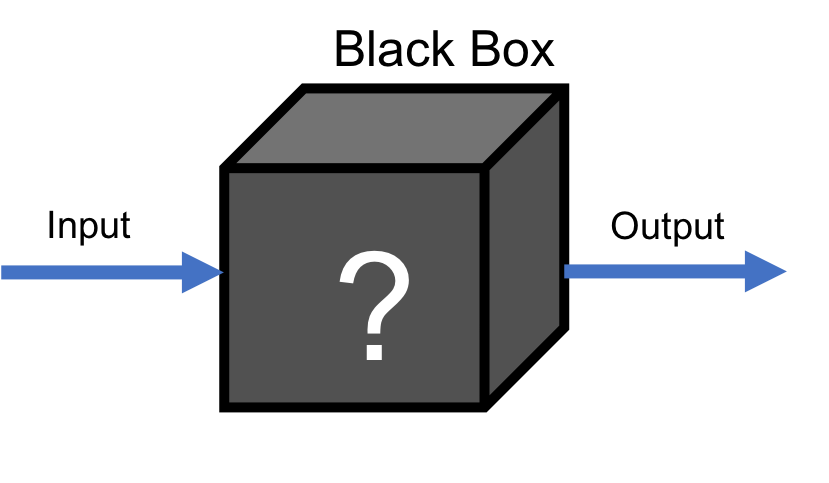
\includegraphics[width=.8\linewidth]{images/black_box.png}
		\label{fig:blackBox}
	\end{subfigure}%
	\begin{subfigure}{.5\textwidth}
		\centering
		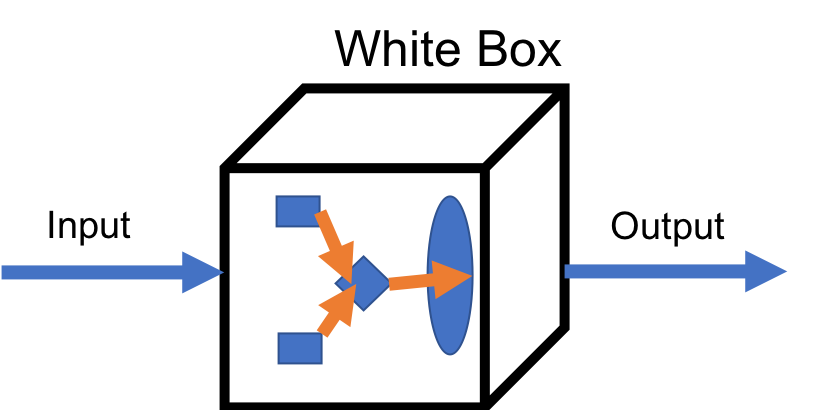
\includegraphics[width=.8\linewidth]{images/white_box.png}
		\label{fig:whiteBox}
	\end{subfigure}
	\caption{A black box scanner derives behaviour strictly from I/O, whilst a white box scanner has all the inner workings of a (web) application at its disposal for analysis}
	\label{fig:test}
\end{figure}


 A white box scanner takes into consideration the implementation of the service, so it may be designed with the specific framework or language used for the application in mind. Conversely, a black box implementation does not care about these details and looks only at outputs from the service. A major differentiation between the two approaches is their use case; a white box scanner emulates the experience of a web developer who is looking to detect potentially exposed parts of his code, whereas a black box scanner portrays the setting for a malicious attacker, where they are only working with the exterior interface of the application to forge an intrusion. The black box approach is the one I will be using in the extension implementation as it aligns best with the project requisites.

\subsection{Related work}
 
A large majority of web vulnerability scanners are designed to be ran passively. This means an auditor of the security of a web application would start the tool, and depending on the length and intensity of the scan, either grab a coffee while it executes or leave it running overnight. Either way, these are expected to produce reports on where a website is suffering from a vulnerability, which can then be interpreted to produce a fix. This automation is a great bonus because it makes life easier for the auditor, as they can get on with other tasks in the meantime; depending on the initial monetary and time investment needed to set up the scan, doing so automatically can be a cost-effective solution for many businesses. \\

There have been studies committed to evaluate the effectiveness of these black box scanners. Doup\'e, Cova and Vigna did an extensive analysis of the tools available in 2010 \cite{whyJohnnyCantPentest}, including tools ranging from free to \$30,000+ worth. In the same year, Bau, Bursztein, Gupta and Mitchell published their own paper with a similar analysis \cite{stateOfArtAutomatedBlackBoxWebAppVulnTesting}. More recently, in 2015, Parvez, Zavarsky and Khoury released a study on the effectiveness of scanners in detecting a limited set of vulnerabilities \cite{analysisOfEffectivenessOfBlackBoxWebAppScannersStoredSQLStoredXSS}. \\

Doup\'e et al. found that \textit{crawling} was one of the major limiting factors of web vulnerability scanners; according to them, {"...crawling is arguably the most important part of a web application vulnerability scanner; if the scanner’s attack engine is poor, it might miss a vulnerability, but if its crawling engine is poor and cannot reach the vulnerability, then it will surely miss the vulnerability"}. To better understand this, it is important to contextualise what \textit{crawling} is. \\

A typical vulnerability scanner will loosely consist of 3 different modules:

\begin{itemize}
	
	\item \textit{Crawling module} - This is the first part of the scanner that gets executed. A crawler will recursively follow every possible link in a webpage so that the tool can build up an internal representation / database of what the target website looks like. As mentioned above, this stage will make or break the scan - though it is unlikely that a crawler will be able to find 100\% of the available subpages on the target website, any missed links will result in the scanner not considering those pages, which in the worst case scenario may miss a page which is the root of many vulnerabilities on the target site. Acunetix themselves, the providers of the commercial vulnerability scanner, say "if you can't crawl it, you can't scan it!" \cite{acunetixQuoteCrawling}. 
	
	\item \textit{Attacker module} - At this stage, the scanner attempts to chip away at any potential cracks in the website. It goes through every stored entry in the previous phase and scans the content of the associated page. Depending on this content (e.g. a form or a URL parameter), the scanner issues web requests with specially crafted input designed to create \textit{interesting} responses from the web server.
	
	\item \textit{Analysis module} - This module reads the outputs from the target to the attacker module input, and scans for any significant or telling change from the server side response. If the web server generates a wildly different response to a normal input (e.g. it issues a page containing an SQL error message), then this is flagged up as a potential vulnerability. This module can have a feedback loop to the attacker module to refine attack methods. This is done through \textit{fuzzing} - creating mutations of the benign input and testing these on the application until a more malicious input is generated that triggers a vulnerability. The scan completes after all potential mutations and attack vectors have been exhausted, or a resource cap is met (time elapsed, bytes sent etc).
\end{itemize}


\begin{figure}[h]
	\centering
	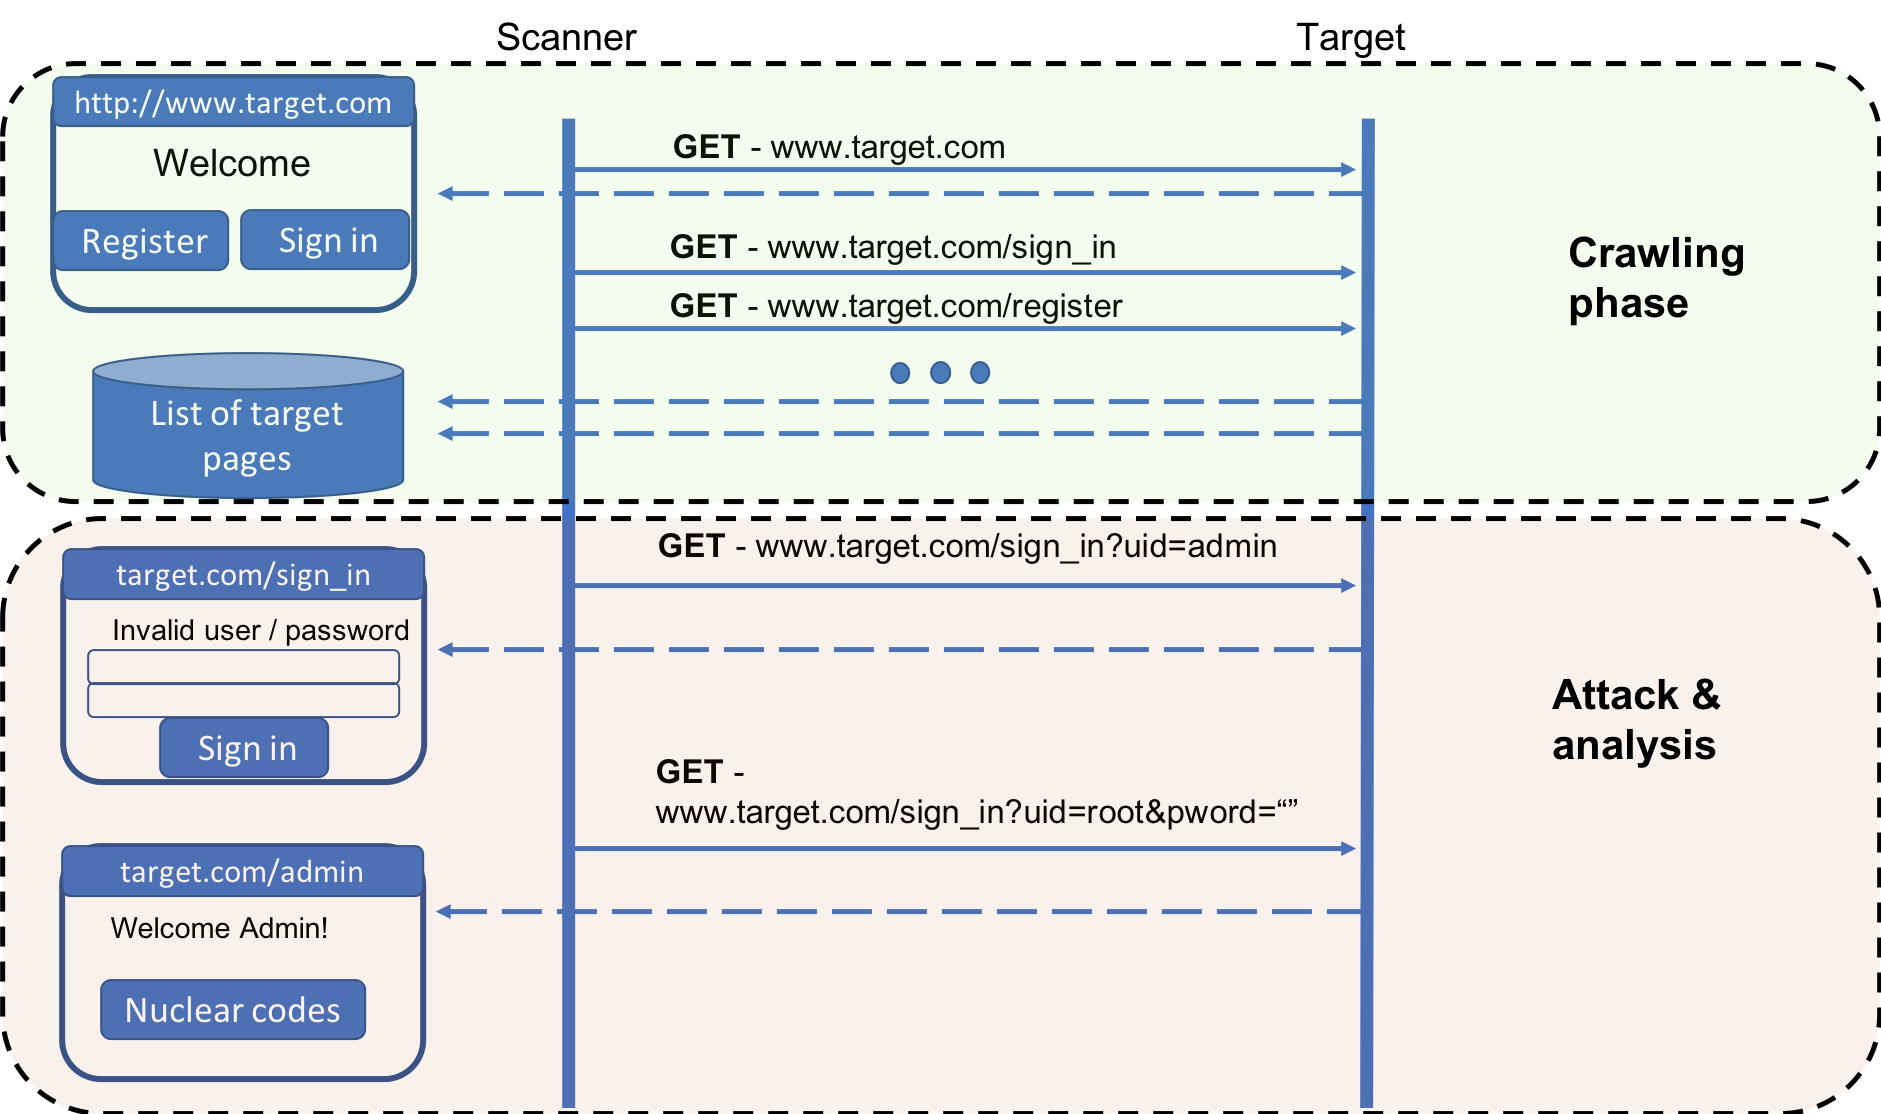
\includegraphics[width=\textwidth]{images/scanner_structure.png}
	\caption{The typical structure of a vulnerability scanner. The crawling phase builds up a database of potential pages to attack. During attack, malicious inputs are fired towards pages to try and trigger undesired behaviour - the analyser reads response contents with some heuristics to determine what responses seem to indicate vulnerabilities.}
	\label{fig:test}
\end{figure}

With this knowledge in mind, it is now easier to appreciate how important the crawling phase is, as it sets an upper bound to how far a scanner can go. Crawling in itself is however not a trivial task to implement. A naive approach to this would be to start at the target page given, scan for any \texttt{<a>} anchor links in this page and filter this list to only include links that belong to the target domain (e.g. if our target was \texttt{facebook.com}, we might be interested in \texttt{facebook.com/account}, but we would discard any links to \texttt{google.com}, as Google links belong to a different domain. As a general rule of thumb, the links we explore have the target link as a prefix to the URL). This method of crawling pages would quickly come up against issues though. A lot of the interesting state of a web application is often hidden behind a login form, so if a valid user account isn't created then a scanner will not be able to explore the full array of actions available. The method described above would not consider this, so would skip out on all the intriguing parts of a website that requires you to have an account. There are also other technologies used in the web that make this slightly harder, such as Flash objects that contain useful sublinks. These objects are not straightforward to analyse, and make automated crawling difficult. \\

This combination of components quickly complicates things for creation of an effective crawler implementation. A competent crawler needs to go above and beyond being just a database of pages - it has to emulate human interactions with an application without any prior domain knowledge. To do so, it has to somehow derive an internal representation of what the website looks like, and refer to this state when crawling and in the analysis phase. Keeping state was an issue raised by Doup\'e et al. in \cite{whyJohnnyCantPentest}. As an example of its importance, if during the attacking phase the scanner is logged in, and an attack request causes the scanner to log out of the application, all the subsequent requests will execute in a different context where the scanner is logged out, invalidating their intended purpose. Doup\'e, Cavedon, Kruegel and Vigna later addressed this by creating a scanner that generated an internal state machine representation of a web application based on heuristically unique server responses \cite{stateAwareBlackBoxWebVulnScanner}. The techniques demonstrated in that paper were useful in creating a more effective crawler that remembered state so as to not waste computation efforts. The resulting scanner achieved higher code coverage rates for web applications analysed over other otherwise similar, open-source scanners. Higher code coverage rates mean that a scanner is exercising more of the application's source code, thus increasing likelihoods of finding a vulnerability. \\

It is clear that an automated crawler based web vulnerability scanner is a difficult tool to create. The shotgun approach used by the crawler can also have negative consequences for the application as discussed in \ref{ethics}. Though state of the art crawlers can now handle the aforementioned hurdles and other intricacies of different web applications, the creation of an efficient, fully automated crawler could warrant a project of its own. \\

These points lead us nicely onto the intended innovation behind the project idea - to create a semi-automated web application vulnerability scanner. The essential difference between this and the aforementioned black box scanners is that it intends to work as an aide alongside a pentester, not as a fully automated background process. 

why should you use human input:
organic, realistic experience
make use of the entire webpage - no need to skip AJAX, JS, flash etc - although these might be out of scope of the project

 using the website as intended allows us to keep a simpler representation of the website
if the scanner works at the same level as the user then they 
 
whyJohnny found that a bunch of students with some knowledge had better results than scanners
 
 Human judgement is needed anyway - scanner won't know for sure. It's a human process to hack, and people will spend hours in crafting specialised attacks. 
 
 "C) Adding interactive multistep options to scan. Out of the three scanners, only one scanner had that feature. While the option to set login credentials helps to provide application’s login info for the scanning, it does not instruct the scanners how to visit the pages and where to put attack vectors to exploit and to detect the vulnerabilities." - Analysis of effectivness of black box web app scanners 
 
 
 "Our experimental findings confirmed that choosing the right attack vectors for the detection and exploitation of stored XSS and stored SQLI remains a big challenge for black box scanners." - Analysis of effectiveness of black box web application scanners in detection of stored sql injection and stored xss vulnerabilities (2015)
 
 "Scanners need to be improved to use right attack vectors in the right situations" - Analysis of effectiveness of black box web application scanners in detection of stored sql injection and stored xss vulnerabilities (2015)
 
\section{Browser extensions}
 
 
 
 
 

 
\section{Limitations}

crawling does find more stuff to look through
\subsection{Human review}

 \subsection{Breadth of  work}
 
 \subsection{Self security}
 	 My own extension is not free from attacks / bugs
http://slideplayer.com/slide/4352044/

\subsection{Ethics \& Handling of Results}
\label{ethics}
 each potential vulnerability may have 100's of different known alternatives to fuzz through,
scans might take the website down if intensive
 
